\chapter{O método dos elementos virtuais}
\label{cap:4}

\section{Introdução ao método dos elementos virtuais}

    \indent Neste capítulo apresenta-se a formulação do Método dos Elementos Virtuais (MEV) aplicada a problemas elastodinâmicos bidimensionais. São desenvolvidos os espaços de aproximação, os operadores de projeção (elíptico, \(L^2\) e de deformações) e as matrizes de rigidez e de massa, com especial ênfase na construção dos projetores de forma generalizada para qualquer ordem de aproximação \(k\). Ao final, discute-se a implementação computacional do método.
    \indent O MEV, similar ao MEF, é uma técnica numérica voltada à solução de equações diferenciais mediante a divisão do domínio em parcelas menores e mais simples de serem solucionadas. A principal característica do MEV é a possibilidade de utilizar funções de base que não são necessariamente polinômios, mas sim funções suaves — soluções de problemas de EDP no interior do elemento. Unindo isso ao aspecto da geometria do elemento ser indiferente à quantidade de nós no elemento permite a existência de elementos diversos em uma mesma malha como pode ser observado na Figura~\ref{fig:4.1}.

    \begin{figure}[H]
        \centering
        \caption{Malha voronoi com elementos em formato de animais.}
        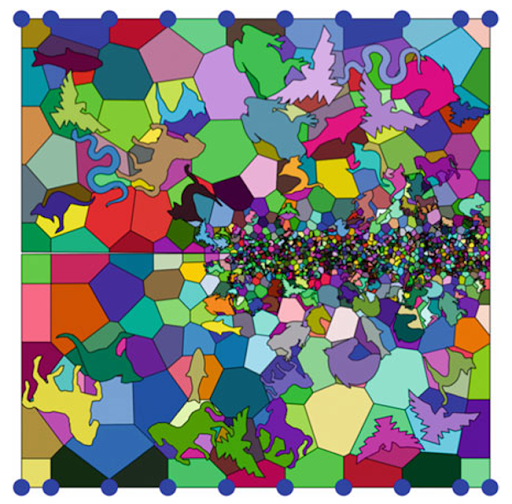
\includegraphics[width=0.8\textwidth]{figuras/Capítulo 4/4.1.png}
        \label{fig:4.1}

        {\small \textbf{Fonte:} \citet{virtualelementformulationphasefieldmodelingductilefracture2019}}
    \end{figure}

    \indent O método foi projetado para lidar com discretizações politopais de formato arbitrário, o que é particularmente conveniente na construção de malhas para geometrias complexas. Ele provou-se robusto ao lidar com malhas de formatos arbitrários, mesmo aquelas com arestas que possuem ângulos de 180° (Figura~\ref{fig:4.2a}) ou ângulos convexos (Figura~\ref{fig:4.2b}). Como destacado por \citet{engineeringperspectivevirtualelementmethoditsinterplaystandardfiniteelementmethod2019a}, a geração e reconstrução de malhas com a correção dos elementos com grandes distorções é um processo que consome tempo na etapa de pré-processamento do MEF, etapa que o MEV permite desconsiderar. 

    \begin{figure}[H]
        \centering
        \caption{Elementos com arestas com ângulos de 180° e convexo.}
        \label{fig:4.2}
        \begin{subfigure}[b]{0.45\textwidth}
            \centering
            \caption{Elemento com ângulos de 180°.}
            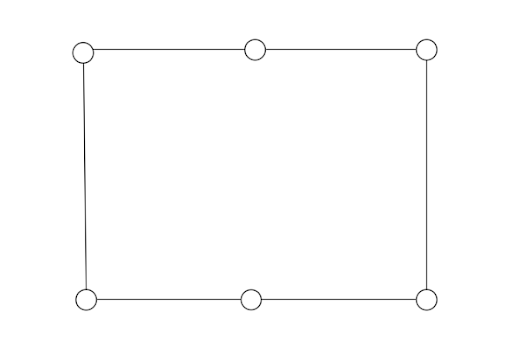
\includegraphics[width=\textwidth]{figuras/Capítulo 4/4.2a.png}
            \label{fig:4.2a}
        \end{subfigure}
        \hfill
        \begin{subfigure}[b]{0.4\textwidth}
            \centering
            \caption{Elemento com ângulo convexo.}
            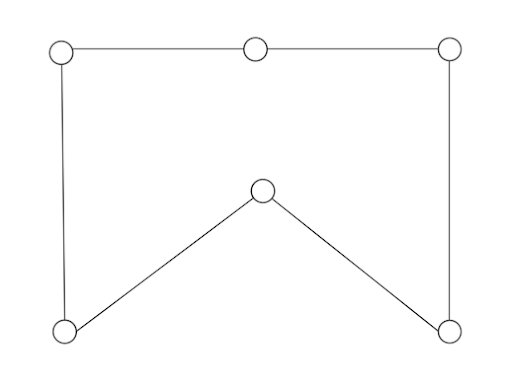
\includegraphics[width=\textwidth]{figuras/Capítulo 4/4.2b.png}
            \label{fig:4.2b}
        \end{subfigure}
        
        {\small \textbf{Fonte:} Elaborado pelo autor (2026).}
    \end{figure}


	\indent O motivo do nome "virtual" é porque as funções de base utilizadas na aproximação não são conhecidas explicitamente. Segundo \citet{vem2017virtual}, "A cada conjunto de graus de liberdade, associamos uma função que não é necessariamente um polinômio, mas sim uma função suave — uma solução de um problema de EDP no interior do elemento". Essa definição é crucial para a distinção entre o MEV e o MEF, no qual as funções de base estão estritamente atreladas à forma do elemento. \\
    \indent Um domínio $\Omega \subset \mathbb{R}^2$ é particionado em um conjunto de elementos poligonais arbitrários não sobrepostos, $\Omega_v$, com contorno $\partial \Omega_v$ composto por arestas retas $e_i$, cujos vértices $V_i$ são denominados nós. O diâmetro, as coordenadas do centroide e a área de um elemento $\Omega_v$ são dados, respectivamente, por $h_E$, $\bar{\mathbf{x}} = (\bar{x}, \bar{y})$ e $\vert{}\Omega_v\vert{}$. 
    
    \begin{figure}[H]
        \centering
        \caption{Geometria de um elemento poligonal.}
        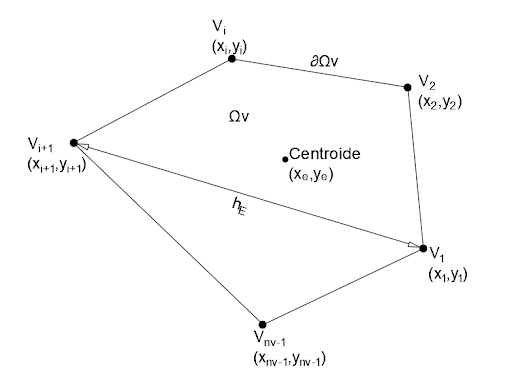
\includegraphics[width=0.7\textwidth]{figuras/Capítulo 4/4.3.png}
        \label{fig:4.3}
        {\small \textbf{Fonte:} Elaborado pelo autor (2026).}
    \end{figure}

    \indent \citet{virtualelementmethod50linesmatlab2017} mostra como são calculadas a área e o centroide de um polígono. A área de um polígono é obtida através das coordenadas dos vértices e o número de vértices $n_v$ utilizando a fórmula:
    
    \begin{equation}
        \vert{}E\vert{} = \frac{1}{2} \left\vert{} \sum_{i=1}^{n_v-1} (x_i y_{i+1} - y_i x_{i+1}) + (x_{n_v} y_1 - x_1 y_{n_v}) \right\vert{},
        \label{eq:4.1}
    \end{equation}

    \noindent Conhecida a área do polígono, as coordenadas do centroide podem ser obtidas por:
    
    \begin{equation}
        \begin{split}
            \bar{x}=\frac{1}{6\vert{}E\vert{}}\left[\sum_{i=1}^{n_v-1}(x_i+x_{i+1})(x_iy_{i+1}-x_{i+1}y_i)+(x_{n_v}+x_1)(x_{n_v}y_1-x_1y_{n_v})\right] \\
            \bar{y}=\frac{1}{6\vert{}E\vert{}}\left[\sum_{i=1}^{n_v-1}(y_i+y_{i+1})(x_iy_{i+1}-x_{i+1}y_i)+(y_{n_v}+y_1)(x_{n_v}y_1-x_1y_{n_v})\right].
        \end{split}
        \label{eq:4.2}
    \end{equation}

    \indent O diâmetro do elemento é a maior distância entre dois vértices, e pode ser obtido com o Algoritmo~\ref{alg:diametro_elemento}:

    \begin{algorithm}[H]
        \caption{Cálculo do diâmetro de um elemento}
        \label{alg:diametro_elemento}
        \begin{algorithmic}[1]
            \Require Conjunto de vértices do elemento $E$: $\mathcal{V}_E = \{\mathbf{x}_1, \dots, \mathbf{x}_{n_v}\}$
            \Ensure Diâmetro $h_E = \max_{\mathbf{x}_i, \mathbf{x}_j \in \mathcal{V}_E} \|\mathbf{x}_i - \mathbf{x}_j\|$

            \State $h_E \gets 0$
            \For{$i \gets 1$ \textbf{to} $n_v - 1$}
                \For{$j \gets i + 1$ \textbf{to} $n_v$}
                    \State $h_E \gets \max\bigl\{h_E,\, \|\mathbf{x}_i - \mathbf{x}_j\|\bigr\}$
                \EndFor
            \EndFor
            \State \Return $h_E$
        \end{algorithmic}
    \end{algorithm}

    \indent \citet{manzini2017annotations} explica que apesar das funções de base não serem polinomiais, elas podem ser separadas em duas partes: a primeira parte representa a solução aproximada por um polinômio de ordem $k$, e a outra corresponde a um complemento composto por funções desconhecidas de natureza não polinomial: 

    \begin{equation}
        \varphi=\Pi_k^{\nabla}\varphi+(I-\Pi_k^{\nabla})\varphi
        \label{eq:4.3}
    \end{equation}

    \indent O MEV é construído de modo que a solução do problema possa ser obtida mesmo sem saber qual é a parcela exata do complemento. Como o método é mapeado por meio funções polinomiais, introduz-se uma base polinomial $\{\mathbf{p}_\alpha\}_{\alpha = 1,...,n_k}$ pertencente ao espaço de polinômios de ordem $k$ no elemento $\Omega$, $\mathbb{P}_{k}(\Omega)$. \citet{vem2017virtual} mostra que a dimensão do espaço de um polinômio de grau $k$ para problemas em $\mathbb{R}^2$ é obtida por: 

    \begin{equation}
        n_k = \frac{(k+1)(k+2)}{2}
        \label{eq:4.4}
    \end{equation}

    \indent Em formulações de elementos virtuais, é muito comum a utilização de bases ao invés de uma expansão polinomial pura. \citet{wriggers2024virtual} Comenta que o uso de bases é frequente na literatura de elementos virtuais para construir matrizes tangentes com valores de condicionamento reduzidos, sendo os monômios escalados uma das bases mais utilizadas. "Eles são uma base centrada no centroide do elemento onde cada coordenada é escalada pelo inverso do diâmetro do elemento, por exemplo, coincidindo com a base canônica em um politopo centrado na origem e escalado para ter diâmetro unitário" (\citet{virtualelementmethodoverviewformulations2024a}). Definem-se os monômios escalados por: 

    \begin{equation}
        \xi = \left( \frac{x - \bar{x}}{h_E} \right) \hspace{1cm} \eta = \left( \frac{y - \bar{y}}{h_E} \right)
        \label{eq:4.5}
    \end{equation}

\section{O elemento virtual}
	
    \indent Os graus de liberdade de um elemento virtual estão relacionados aos nós do elemento, que correspondem aos vértices do polígono e aos $k-1$ pontos intermediários ao longo das arestas, e, variáveis internas-- chamadas momentos internos-- em aproximações de alta ordem, assumindo valores escalares ou vetoriais. 

    \begin{figure}[htbp]
        \centering
        \caption{Elemento virtual.}
        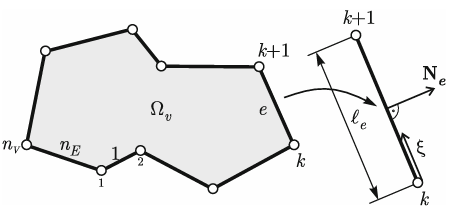
\includegraphics[width=\textwidth]{figuras/Capítulo 4/4.4.png}
        \label{fig:4.4}
        {\small \textbf{Fonte:} \citet{wriggers2024virtual}}
    \end{figure}


    \indent Cada aresta do elemento é descrita por um polinômio de grau $k$ e, de forma similar aos elementos finitos, é mapeada através dos nós. Quando $k > 1$, é necessário adicionar $k - 1$ nós intermediários, igualmente espaçados, ao longo de cada aresta. \\
    \indent Na solução de problemas com aproximação de ordem $k > 1$, surgem termos no interior do elemento que não podem ser calculados explicitamente. Uma maneira de contornar isso é torná-los graus de liberdade do problema, denominados momentos internos. Essas variáveis surgem como forma de tratar a indeterminação da formulação, que será visto durante o cálculo dos operadores de projeção na secção~\ref{sec:projetor elíptico}, e possuem a forma: 

    \begin{equation}
        \mathbb{m} = \frac{1}{\vert{}\Omega_v\vert{}}\int_\Omega p\,v_h\,d\Omega\quad\forall\,p\in\mathbb{P}_{k-2}(\Omega)
        \label{eq:4.6}
    \end{equation}

	\indent A quantidade de graus de liberdade por elemento com $n_v$ vértices e ordem $k$ em problemas vetoriais em duas dimensões é distribuída da seguinte forma: 
    
    \begin{itemize}
        \item Vértices: $2 n_v$ 
        \item Arestas: $2 n_v (k - 1)$
        \item Interior: $k^2 - k$
    \end{itemize}

    \indent A Figura~\ref{fig:4.5} apresenta a disposição dos graus de liberdade deste tipo de problema para ordens de interpolação $k = 1, 2, 3$. Na figura cada nó representado possui dois graus de liberdade.

    \begin{figure}[htbp]
        \centering
        \caption{Geometria do elemento.}
        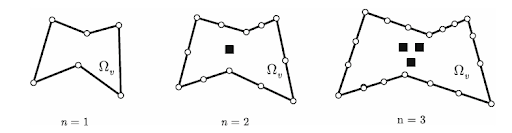
\includegraphics[width=\textwidth]{figuras/Capítulo 4/4.5.png}
        \label{fig:4.5}
        {\small \textbf{Fonte:} \citet{wriggers2024virtual}}
    \end{figure}

\section{Espaço de solução}

	\indent Apesar de não serem conhecidas explicitamente, as funções virtuais são representadas por meio de suas projeções sobre espaços polinomiais. Para isso, constrói-se um operador de projeção que permite extrair a componente polinomial da solução. Na formulação clássica do MEV, a parte polinomial garante a consistência do método, enquanto a parcela não polinomial assegura a estabilidade da formulação.\\
    \indent No MEV, o espaço local de aproximação não pode ser escrito de forma explícita. Para o problema elastodinâmico, a formulação é construída de modo a garantir continuidade $C^0$ entre os elementos nos nós e arestas, isto é, as variáveis de campo (os deslocamentos) são contínuas através das interfaces e, em cada aresta, correspondem a polinômios de grau $k$. Para o contorno de um elemento $\Omega_v$ com arestas $e$, define-se o espaço auxiliar

    \begin{equation}
        \mathbb{B}_k(\partial \Omega_v) := \bigl\{v \in C^0(\partial \Omega_v) : v|_{e} \in \mathbb{P}_k(e)\quad \forall\, e \subset \partial \Omega_v\bigr\}.
        \label{eq:4.7}
    \end{equation}

    \indent No interior do elemento, exige-se apenas que o laplaciano pertença ao espaço dos polinômios de grau no máximo $k-2$. Desse modo, o espaço local de aproximação é definido por

    \begin{equation}
        \mathbb{V}^{\Omega_v,k} := \bigl\{v \in H^1(\Omega_v) : v|_{\partial \Omega_v} \in \mathbb{B}_k(\partial \Omega_v), \quad \nabla^2 v|_{\Omega_v} \in \mathbb{P}_{k-2}(\Omega_v)\bigr\}.
        \label{eq:4.8}
    \end{equation}

    \indent Como observado por \citet{basicprinciplesvirtualelementmethods2013a}, outros operadores diferenciais de segunda ordem poderiam ser utilizados no lugar do laplaciano. Contudo, tanto para a equação de Laplace quanto para a equação do movimento tratada neste trabalho, a escolha do operador de Laplace é a mais natural (essa escolha será justificada na Seção~\ref{sec:projetor elíptico}). Como o laplaciano da função virtual é, por definição, um polinômio de grau $\le k-2$, no caso de aproximação de primeira ordem ($k=1$) tem-se $\nabla^2 v = 0$. As funções no interior do elemento são, portanto, harmônicas\footnote{Diz-se que uma função $v$ é harmônica em um domínio quando satisfaz a equação de Laplace homogênea, isto é, $\nabla^2 v = 0$ no interior do domínio (para uma revisão formal, ver \citet[Capítulo~2]{evans2010partial}). O termo ``harmônica'' remete historicamente às soluções baseadas em funções senoidais que descrevem modos de vibração e oscilações acústicas, propriedades que se generalizam para as soluções de menor energia associadas ao operador de Laplace.}.\\
    \indent Como brevemente comentado na introdução do capítulo, as funções virtuais são, por construção, soluções de problemas de contorno locais. De fato, a unisolvência e a dimensão correta do espaço $\mathbb{V}^{\Omega_v,k}$ decorrem diretamente do fato de que, para cada par $(g,q)$ com $g\in\mathbb{B}_k(\partial \Omega_v)$ e $q\in\mathbb{P}_{k-2}(\Omega_v)$, o problema

    \begin{equation*}
        \begin{cases}
            \Delta v = q & \text{em }\Omega_v,\\
            v = g & \text{em }\partial \Omega_v,
        \end{cases}
    \end{equation*}

    \noindent admite solução única em $H^1(\Omega_v)$. Assim, cada escolha do par $(g,q)$ determina exatamente uma função do espaço virtual.\\
    \indent A notação \(H^1(\Omega)\) designa o espaço de Sobolev de ordem 1. De acordo com \citet{hughes1987finite}, os espaços de Sobolev \(H^n(\Omega)\) são constituídos por funções que, juntamente com todas as suas derivadas fracas até a ordem \(n\), pertencem a \(L^2(\Omega)\). Isso significa que as funções pertencentes a \(H^1(\Omega)\), bem como as suas derivadas de primeira ordem, são de quadrado integrável. A forma variacional da equação do movimento (Eq.~\ref{eq:3.58}) envolve apenas derivadas de primeira ordem na parcela elástica; portanto, o espaço natural de busca da solução é \(H^1(\Omega)\). Uma função \(f\) é dita de quadrado integrável quando

    \begin{equation}
        \|f\|_{L^2(\Omega)}^2 = \int_{\Omega} |f|^2 \, d\Omega < \infty.
        \label{eq:4.9}
    \end{equation}

    \indent A exigência de que as funções de aproximação sejam de quadrado integrável está diretamente relacionada à existência, unicidade e estabilidade da solução do problema discreto. Ao se aplicar uma função polinomial e as suas derivadas na Eq.~\ref{eq:4.9}, verifica-se que a integral permanece finita, o que justifica o emprego de funções polinomiais como base de aproximação.\\
    \indent O espaço de soluções definido na Eq.~\ref{eq:4.8} permite a construção de um operador de projeção para o gradiente (e para outros operadores diferenciais de primeira ordem) das funções de base com boa precisão. Por essa razão, ele é adequado para a aproximação dos termos de tipo \(H^1\) da equação diferencial. No entanto, quando se deseja projetar diretamente as próprias funções de base -- e não apenas os seus gradientes -- a projeção apresenta erros significativos. Isso prejudica a aproximação dos termos de tipo \(L^2\), como o termo de massa e o termo de força. Para contornar essa limitação, \citet{equivalentprojectorsvirtualelementmethods2013a} introduziram um espaço de soluções aumentado, baseado em uma projeção \(L^2\), definido por

    \begin{equation}
        \begin{aligned}
            V^{\Omega_v,k} := \Bigl\{ v \in H^1(\Omega_v) :\;& v\big|_{\partial\Omega_v} \in \mathbb{B}_k(\partial\Omega_v),\; \nabla^2 v\big|_{\Omega_v} \in \mathbb{P}_k(\Omega_v), \\ & \int_{\Omega_v} \bigl(v - \Pi_k^{\nabla} v\bigr)\,\mu \,d\Omega_v = 0 \quad \forall\,\mu \in \mathbb{P}_k(\Omega_v)\setminus\mathbb{P}_{k-2}(\Omega_v)\Bigr\}.
        \end{aligned}
        \label{eq:4.10}
    \end{equation}

    \indent Esse espaço apresenta como característica o laplaciano de uma função pertencer ao espaço $\mathbb{P}_k(\Omega)$, em contraste com a definição clássica em que deve estar em $\mathbb{P}_{k-2}(\Omega)$ e um termo extra, cujo propósito será esclarecido na secção~\ref{sec:Projetor L2}. Na formulação estendida, os graus de liberdade coincidem com os do espaço clássico apresentando a propriedade: 

    \begin{equation}
        \int_{\Omega_v} w_h p_\alpha d\Omega_v = \int_{\Omega_v} \Pi^\nabla w_h p_\alpha d\Omega_v, \hspace{5mm} \vert{}\alpha\vert{} = k-1,k 
        \label{eq:4.11}
    \end{equation}

\section{Operadores de projeção}
\label{sec:operadores-de-projecao}

    \indent Como o espaço de soluções não é explicitamente conhecido, operadores de projeção são utilizados para capturar a parte polinomial das funções de base. Os operadores de projeção são mapeamentos lineares cuja imagem corresponde à parcela polinomial do espaço de soluções. Para cada elemento, constrói-se uma matriz cujos coeficientes correspondem aos termos de uma expansão polinomial. Define-se o espaço polinomial escalar $\mathbb{P}_k(\Omega_v)$ através do \textit{span} da base de monômios escalados:
    
    \begin{equation}
        \mathbb{P}_k(\Omega_v) = \operatorname{span} \{ p_\alpha \}_{\alpha=1}^{n_k} = \operatorname{span} \{ 1, \xi, \eta, \xi^2, \xi \eta, \dots, \eta^k \},
        \label{eq:4.12}
    \end{equation}
    cujos elementos são organizados no vetor $H_k^{P} \in \mathbb{P}_k(\Omega_v)$:
    \begin{equation}
        H_k^{P} = \begin{Bmatrix} 1 & \xi & \eta & \xi^2 & \xi \eta & \ldots & \eta^k \end{Bmatrix}.
        \label{eq:4.13}
    \end{equation}

    \vspace{5mm}
    \fbox{ \begin{minipage}{0.8\textwidth} 
    \textbf{Exemplo 4.1.} Para uma aproximação quadrática, construa o vetor $H_2^{P}$.
    
    \hrulefill
    
    Solução:\\[3mm]
    $H_2^{P} = \begin{Bmatrix} 1 & \xi & \eta & \xi^2 & \xi \eta & \eta^2 \end{Bmatrix}$. 
    \end{minipage} }\vspace{5mm}

    \indent Como o projetor resulta em uma função polinomial, a projeção das funções de base $\varphi$ pode ser descrita por: 

    \begin{equation}
        \Pi \varphi = \left( H_k^{P} \right)^T \{a\},
        \label{eq:4.14}
    \end{equation}
    
    \noindent onde $\{a\}$ representa o vetor de coeficientes escalares.\\  
    \indent Em problemas vetoriais com dois graus de liberdade por nó ($u$ e $v$), o espaço de aproximação é $[\mathbb{P}_k(\Omega_v)]^2$. Adotando a ordenação intercalada para os graus de liberdade de deslocamento ($u$ e $v$), o \textit{span} do espaço polinomial vetorial é construído alternando as componentes horizontal e vertical para cada monômio: 

    \begin{equation}
        \begin{aligned}
            \relax [\mathbb{P}_k(\Omega_v)]^2 = \operatorname{span} \left\{ \begin{Bmatrix} p_\alpha \\ 0 \end{Bmatrix}, \begin{Bmatrix} 0 \\ p_\alpha \end{Bmatrix} \right\}_{\alpha}^{n_k} = \\ \operatorname{span} \left\{ \begin{Bmatrix} 1 \\ 0 \end{Bmatrix}, \begin{Bmatrix} 0 \\ 1 \end{Bmatrix}, \begin{Bmatrix} \xi \\ 0 \end{Bmatrix}, \begin{Bmatrix} 0 \\ \xi \end{Bmatrix}, \begin{Bmatrix} \eta \\ 0 \end{Bmatrix}, \begin{Bmatrix} 0 \\ \eta \end{Bmatrix}, \dots, \begin{Bmatrix} \eta^k \\ 0 \end{Bmatrix}, \begin{Bmatrix} 0 \\ \eta^k \end{Bmatrix} \right\}.
        \end{aligned}
        \label{eq:4.15}
    \end{equation}

    \indent Essa construção garante o desacoplamento cinemático entre os campos de deslocamento $u_h$ e $v_h$, assegurando a independência linear dos coeficientes de expansão de cada direção. Assim, para cada monômio escalar $p_\alpha$, o índice $\alpha$ da base vetorial associa-se a um par de vetores na base.\\
    \indent As funções de base, $\varphi$, não necessitam ser explicitadas no interior do elemento, pois são definidas diretamente pela relação com os funcionais de grau de liberdade, $\chi_i$. Essa relação estabelece a base canônica:
    \begin{equation}
        \chi_i(\varphi_j) = \delta_{i,j}.
    \end{equation}
    \noindent Consequentemente, qualquer campo de deslocamentos aproximado $u_h$ é expresso pela expansão do tipo Lagrangiana:
    \begin{equation}
        u_h = \sum_{i=1}^{n_{\mathrm{dof}}} \chi_i(u_h) \, \varphi_i.
        \label{eq:4.16}
    \end{equation}

    \indent Embora o campo $u_h$ seja virtual no domínio, seus valores no contorno são conhecidos. Conforme definido na Eq.~\ref{eq:4.8}, o traço do deslocamento sobre uma aresta $e \subset \partial \Omega_v$, denotado por $\left. u_h \right|_{\partial \Omega_v}$, é um polinômio de grau $k$ interpolado pelos $k+1$ nós contidos em cada aresta:
    \begin{equation}
        \left. u_h \right|_{\partial \Omega_v}(\xi) = \sum_{j=1}^{k+1} M_j(\xi) \, u_j^{(e)},
        \label{eq:4.17}
    \end{equation}
    \noindent $M_j(\xi)$ são funções de interpolação nodais nas arestas, parametrizada pela coordenada local $\xi \in [0, 1]$, e $u_j^{(e)}$ são os valores das variáveis de campo nos nós de uma aresta $e$. Dessa forma, a restrição de uma função de base global $\varphi_i$ à aresta $e$ reduz-se à função de interpolação unidimensional $M_i(\xi)$ para os nós situados sobre essa aresta e anulando-se para os demais graus de liberdade do elemento:
    \begin{equation}
        \varphi_{i|\partial \Omega_v}(\xi) = M_{i|\partial \Omega_v}(\xi)
        \label{eq:4.18}
    \end{equation}
    \vspace{5mm}

    \fbox{ \begin{minipage}{0.8\textwidth} 
    \textbf{Exemplo 4.3.} Demonstre a propriedade $\varphi_{i|\partial \Omega_v} = M_{i|\partial \Omega_v}(\xi)$.
    
    \hrulefill
    
    Solução: \\[3mm]
    Cada função de base $\varphi_i$ está associada a um único grau de liberdade. Para $\varphi_i(u_i) = 1$ e $\varphi_i(u_j) = 0$. Sabe-se que: $$u_{h|\partial \Omega_v} = \sum_{j=1}^{k+1} M_j(\xi) u_j.$$ Ao aplicar o somatório para uma função de base $\varphi_i$ na aresta: 
    $$\varphi_{i|\partial \Omega_v}(\xi) = M_1(\xi).0 + \ldots + M_i(\xi).1 + \ldots M_{k+1}(\xi).0 = M_i(\xi).$$
    \end{minipage} }\vspace{5mm}

	\indent Em uma mesma equação diferencial existe diferentes projetores para cada termo da forma variacional, desde que as definições dos espaços de funções (Eq.~\ref{eq:4.8} e Eq.~\ref{eq:4.10}) sejam respeitadas. Existem diversas maneiras de obter os projetores, sendo as duas mais comuns por meio da forma fraca da equação diferencial ou pelo Método de Galerkin. A aproximação via forma fraca exige que a forma bilinear entre a função virtual $v_h$ e uma função teste polinomial $p$ seja equivalente à forma bilinear calculada entre a projeção de $v_h$ e a mesma função $p$: 
    
    \begin{equation}
        a(v_h,p) = a(\Pi v_h,p) \Leftrightarrow \int_\Omega \epsilon(v_h)\mathbb{C} \epsilon(p) d\Omega = \int_\Omega \epsilon(\Pi v_h)\mathbb{C} \epsilon(p) d\Omega \quad \forall p \in [\mathbb{P}_k(\Omega_v)]^2.
        \label{eq:4.19}
    \end{equation}

    \indent A segunda abordagem utiliza o método de Galerkin. Como constatado por \citet{wriggers2024virtual}, a projeção por Galerkin apresenta a vantagem de evitar cinemática e relações constitutivas não lineares. \\
    \indent De modo análogo ao esquema elaborado em \citet{arbitraryorder2dvirtualelementspolygonalmeshespartelasticproblem2017a}, dois operadores distintos serão utilizados para a implementação do problema elastodinâmico: o primeiro é desenvolvido para a matriz de massa e o segundo para a matriz de rigidez. 

\subsection{Projetor \texorpdfstring{$\Pi_{k}^{\nabla}$}{Pi k nabla}}
\label{sec:projetor-eliptico}

    \indent O projetor $\Pi_k^\nabla$ foi desenvolvido em \citet{basicprinciplesvirtualelementmethods2013a} como um dos primeiros operadores de projeção atrelados ao método dos elementos virtuais. Concebido inicialmente para solução do problema de Laplace, esse operador também se aplica a problemas de elasticidade, visto que tanto as tensões quanto às deformações dependem do gradiente. \\
    \indent O desenvolvimento desse projetor é feito por meio da ortogonalização dos gradientes entre a função polinomial e o resíduo da aproximação, procedimento análogo ao do Método de Galerkin 
    
    \begin{equation}
        \int_\Omega \nabla p \cdot \nabla (\varphi - \Pi_k^\nabla \varphi) \, d\Omega = 0 \quad \forall p \in [\mathbb{P}_k(\Omega_v)]^2.
        \label{eq:4.20}
    \end{equation}

    \indent Vetores podem ser decompostos em componentes. Dois vetores são ortogonais entre si quando não possuem componentes em comum. Abstraindo para funções, ao ortogonalizar uma função polinomial de ordem $k$ pelo resíduo das funções de base garante que o resíduo contenha apenas a parcela da solução que não possa ser descrita pela função polinomial. \\
    \indent Aplicando a propriedade de linearidade do operador gradiente, a Eq.~\ref{eq:4.21} escreve-se como: 

    \begin{equation}
        \int_\Omega \nabla p \nabla (\Pi_k^\nabla \varphi)  \, d\Omega = \int_\Omega \nabla p \nabla \varphi  \, d\Omega \quad \forall p \in [\mathbb{P}_k(\Omega_v)]^2.
        \label{eq:4.21}
    \end{equation}

    \indent Em problemas vetoriais bidimensionais, a base de monômios escalados $\mathbb{P}_k(\Omega_v)$ é estendida para o campo vetorial de deslocamentos $[\mathbb{P}_k(\Omega_v)]^2$. A base de monômios vetoriais $H_k^{P}$ é escrita com intercalação das componentes de deslocamento $u$ e $v$, garantindo a ordenação adequada dos graus de liberdade. Substituindo a função polinomial teste pela matriz de monômios $H_k^P$ e expressando o projetor por meio da expansão polinomial, Eq.~\ref{eq:4.14}, tem-se: 
    \begin{equation}
        \int_\Omega \nabla (H^P(\xi,\eta)) \nabla (H^P(\xi,\eta)) \{a\}  \, d\Omega = \int_\Omega \nabla (H^P(\xi,\eta)) \nabla \varphi  \, d\Omega
        \label{eq:4.22}
    \end{equation}

    \indent Como o vetor $\{a\}$ contém coeficientes constantes, ele pode ser retirado da integral: 

    \begin{equation}
        \left(\nabla H_k^P(\xi,\eta), \nabla H_k^P(\xi,\eta) \right)_{\Omega_v}  \{a\} =  (\nabla H_k^P(\xi,\eta), \nabla \varphi)_{\Omega_v} \Leftrightarrow \mathcal{G}^{(\nabla)} \{a\} = \mathcal{B}^{(\nabla)}
        \label{eq:4.23}
    \end{equation}

    \indent O lado esquerdo ($\mathcal{G}^{(\nabla)}$) contém apenas termos polinomiais e pode ser avaliado diretamente via integração numérica (como as técnicas propostas por \citet{bivariatesplineconstructionorthonormalpolynomialspolygonaldomainsitsapplicationsquadrature2026}, \citet{productgausscubaturepolygonsbasedgreensintegrationformula2007}, \citet{calculationarbitrarymomentspolygonsa} e \citet{numericalintegrationpolynomialsdiscontinuousfunctionsirregularconvexpolygonspolyhedrons2011}). Todavia, o lado direito ($\mathcal{B}^{(\nabla)}$) envolve as funções virtuais $\varphi$. Para contornar essa limitação, aplica-se o teorema da divergência: 
    
    \begin{equation}
        (\nabla H_k^P(\xi,\eta) , \nabla \varphi)_{\Omega_v} = \int_{\partial \Omega_v} \left(\nabla H_k^P(\xi,\eta) \cdot \mathbf{n} \right) \varphi_{i\vert{}{\partial \Omega_v}} d{\partial \Omega_v} - \int_{\Omega_v} \nabla^2 (H_k^P(\xi,\eta)) \varphi_i d\Omega 
        \label{eq:4.24}
    \end{equation} 

    \indent A análise da identidade do projetor na Eq.~\ref{eq:4.24} revela de forma direta como o espaço de solução $\mathbb{V}^k$ foi desenhado sob medida para tornar as funções virtuais computáveis sem o conhecimento explícito de seu interior.
    \begin{itemize}
        \item Avaliação do Contorno: A primeira parcela da equação exige o conhecimento da função virtual nas bordas do elemento. Como a definição do espaço restringe $v_{\vert{}\partial \Omega}$ a um comportamento estritamente polinomial, este termo pode ser avaliado de forma exata utilizando os graus de liberdade de fronteira e técnicas padrão de quadratura numérica.
        \item O Laplaciano em $\mathbb{V}^k$: A presença do Laplaciano na definição do espaço $\mathbb{V}^k$ é uma exigência matemática decorrente da solução de problemas elípticos de segunda ordem. Como a forma variacional dessas equações utiliza o produto interno entre gradientes, a aplicação do Teorema da Divergência converte o operador em um Laplaciano ($\nabla \cdot \nabla = \nabla^2$), ditando a restrição teórica exata que o método deve acomodar.
        \item Queda do Grau Polinomial: Na parcela de domínio, a aplicação do operador Laplaciano ($\nabla^2$) sobre a matriz de polinômios $H_k^P$ de grau $k$ reduz o seu grau em duas unidades. O resultado matemático dessa operação recai inevitavelmente sobre o espaço polinomial $\mathbb{P}_{k-2}$.
        \item Momentos Internos: A imposição da condição $\nabla^2 v_{\vert{}\Omega} \in \mathbb{P}_{k-2}(\Omega)$ serve para espelhar a queda de grau descrita acima. Essa restrição calibra a definição dos momentos internos (Eq.~\ref{eq:4.6}), garantindo que a quantidade de graus de liberdade internos gerados seja perfeitamente equivalente à dimensão do espaço $\mathbb{P}_{k-2}$. Assim, o elemento armazena a quantidade exata de informação necessária para solucionar a integral de domínio, sem dados redundantes ou faltantes, assegurando o fechamento do problema local.
    \end{itemize}
    \indent Cada coluna da matriz $\mathcal{B}$ equivale a um grau de liberdade, desse modo, as parcelas das integrais não interagem entre si, com cada uma ocupando colunas distintas da matriz. Ambas as parcelas da Eq.~\ref{eq:4.24}, agora, podem ser resolvidas.\\
    \indent Para a montagem das matrizes do MEV generalizadas para qualquer $k$, algumas considerações em relação aos índices dos graus de liberdade devem ser feitas. O conjunto dos graus de liberdade, $\mathcal{I} = \{1, \dots, n_{\mathrm{dof}}\}$, é particionado em duas contribuições: o contorno ($\mathcal{I}^{(bnd)}$) e o domínio ($\mathcal{I}^{(dom)}$). Essa decomposição estabelece que: $$\mathcal{I} = \mathcal{I}^{(bnd)} \cup \mathcal{I}^{(dom)}, \quad \text{com} \quad \mathcal{I}^{(bnd)} \cap \mathcal{I}^{(dom)} = \emptyset.$$ A relação entre o índice global $i \in \mathcal{I}$ e a geometria do elemento é realizada por meio de duas funções de mapeamento inverso:

\begin{itemize}
    \item \textbf{Função de mapeamento de contorno $\ell_e(i)$:}  
    Dado o índice global $i$, a função $\ell_e(i)$ devolve o índice local do nó na aresta $e$ se $i$ pertencer àquela aresta; caso contrário, devolve um valor inválido (por convenção $0$).

    Para construí-la, utiliza-se a numeração perimetral dos nós. Os nós da fronteira são enumerados sequencialmente em sentido anti-horário. O número do nó local $N_{\text{local}}$ no perímetro, para o $q$-ésimo ponto ($q \in \{1,\dots,k+1\}$) da aresta $e$, é dado por:
    \begin{equation}
        N_{\text{local}}(e, q) = 
        \begin{cases} 
            (e - 1)k + q, & \text{se } q \le k, \\
            e \cdot k + 1, & \text{se } q = k+1 \text{ e } e < n_e, \\
            1, & \text{se } q = k+1 \text{ e } e = n_e \quad (\text{fechamento}).
        \end{cases}
    \end{equation}
    O índice global correspondente a esse nó na direção $d$ é
    \[
    i_e^{(bnd)}(q,d) = \bigl(N_{\text{local}}(e,q) - 1\bigr) \cdot n_{\text{dof\_nó}} + d.
    \]
    Com isso, define-se:
    \[
    \ell_e(i) = 
    \begin{cases}
        q & \text{se existe } q\in\{1,\dots,k+1\} \text{ e direção } d \text{ tais que } i = i_e^{(bnd)}(q,d), \\
        0 & \text{caso contrário.}
    \end{cases}
    \]

    \item \textbf{Função de mapeamento de domínio $m(i)$:}  
    Dado o índice global $i$, a função $m(i)$ devolve o índice do momento interno $\beta$ se $i$ for um grau de liberdade de domínio; caso contrário, devolve $0$.

    Como os graus de liberdade de domínio são ordenados após todos os $N_{\mathrm{bnd}} = n_e \cdot k \cdot n_{\text{dof\_nó}}$ graus de liberdade de contorno, o índice global do $\beta$-ésimo momento interno na direção $d$ é
    \[
    i^{(dom)}(\beta,d) = N_{\mathrm{bnd}} + (\beta - 1) \cdot n_{\text{dof\_nó}} + d.
    \]
    Define-se então:
    \[
    m(i) = 
    \begin{cases}
        \beta & \text{se existe } \beta\in\{1,\dots,n_{k-2}\} \text{ e direção } d \text{ tais que } i = i^{(2)}(\beta,d), \\
        0 & \text{caso contrário.}
    \end{cases}
    \]
\end{itemize}

    \vspace{5mm}
\noindent\fbox{
    \begin{minipage}{0.95\textwidth}
        \textbf{Exemplo 4.x.} Considere um elemento poligonal de $n_e = 4$ arestas com ordem de aproximação quadrática ($k = 2$) e $n_{\text{dof\_nó}} = 2$ graus de liberdade por nó (deslocamentos $u_x$ e $u_y$). Determine os valores das funções de mapeamento para as seguintes situações:

        \textbf{a)} $\ell_3(i)$ no nó intermediário da 3ª aresta ($q = 2$) na direção $y$ ($d = 2$)

        \textbf{b)} $\ell_4(i)$ no ponto final da última aresta ($q = 3$) na direção $x$ ($d = 1$)

        \textbf{c)} $m(i)$ para o primeiro momento interno ($\beta = 1$) na direção $x$ ($d = 1$)

        \hrulefill

        \textbf{Solução:}

        \textbf{a)} Para $e = 3$, $q = 2$ (como $q \le k$):
        \begin{equation*}
            N_{\text{local}}(3, 2) = (3 - 1)\cdot 2 + 2 = 6
        \end{equation*}
        O índice global correspondente é
        \begin{equation*}
            i_3^{(bnd)}(2,2) = (6 - 1)\cdot 2 + 2 = 12.
        \end{equation*}
        Portanto, $\ell_3(12) = 2$ (e $\ell_e(12) = 0$ para $e\neq 3$).

        \textbf{b)} Para $e = 4$, $q = 3$ (fechamento do perímetro):
        \begin{equation*}
            N_{\text{local}}(4, 3) = 1
        \end{equation*}
        O índice global correspondente é
        \begin{equation*}
            i_4^{(1)}(3,1) = (1 - 1)\cdot 2 + 1 = 1.
        \end{equation*}
        Portanto, $\ell_4(1) = 3$ (e $\ell_e(bnd) = 0$ para $e\neq 4$).

        \textbf{c)} O número total de graus de liberdade de contorno é
        \[
        N_{\mathrm{bnd}} = n_e\cdot k\cdot n_{\text{dof\_nó}} = 4\cdot 2\cdot 2 = 16.
        \]
        O índice global do primeiro momento interno na direção $x$ é
        \begin{equation*}
            i^{(dom)}(1,1) = 16 + (1 - 1)\cdot 2 + 1 = 17.
        \end{equation*}
        Portanto, $m(17) = 1$ (e $m(i) = 0$ para qualquer $i$ de contorno).
    \end{minipage}
}
\vspace{5mm}

    \indent Para computar a parcela do domínio, é necessário calcular o Laplaciano da matriz polinomial $H_k^P$. Como a matriz é composta pelo conjunto de polinômios $p_\alpha$, o Laplaciano expressa-se por:
    \begin{equation}
        \nabla^2 p_\alpha = \sum_{\beta=1}^{n_{k-2}} d_{\alpha\beta}\, p_\beta 
        \quad\forall\, p_\alpha\in\mathbb{P}_k(\Omega_v),\; p_\beta\in\mathbb{P}_{k-2}(\Omega_v),
        \label{eq:4.25}
    \end{equation}
    \noindent onde $d_{\alpha\beta}$ representa a matriz de coeficientes do Laplaciano. Substituindo a Eq.~\eqref{eq:4.25} na integral de volume, a parcela do domínio reescreve-se como:
    \begin{equation}
        \int_{\Omega_v}\nabla^2\bigl(H_k^P(\xi,\eta)\bigr)\,\varphi_i\,d\Omega 
        = \sum_{\beta=1}^{n_{k-2}} d_{\alpha\beta}\int_{\Omega_v}p_\beta\,\varphi_i\,d\Omega.
        \label{eq:4.26}
    \end{equation}

    \indent A integral resultante na Eq.~\eqref{eq:4.26} corresponde exatamente à definição dos momentos internos. Destarte, a parcela do domínio é calculada diretamente a partir dos graus de liberdade de volume, prescindindo de integração numérica:
    \begin{equation}
        \int_{\Omega_v}\nabla^2\bigl(H_k^P(\xi,\eta)\bigr)\,\varphi_i\,d\Omega 
        = |\Omega_v|\sum_{\beta=1}^{n_{k-2}} d_{\alpha\beta}\,\delta_{m(i),\,\beta}.
        \label{eq:4.27}
    \end{equation}
    
    \indent A parcela do contorno, por sua vez, é avaliada via integração numérica. Recomenda-se o uso do método de quadratura de Gauss-Lobatto, visto que seus pontos de integração coincidem com os nós do elemento. Como a restrição da função de base global ao bordo da aresta $e$ equivale à base local, tem-se $$ \varphi_{i\big|_{\partial \Omega_v}}(\xi) = M_{\ell_e(i)}(\xi)$$ (quando $\ell_e(i)\neq 0$). A aplicação da quadratura resulta em:
    \begin{equation}
        \sum_{e=1}^{n_e}\int_{\partial \Omega_v}\bigl(\nabla H_k^P\cdot N^{(e)}\bigr)\,\varphi_{i\big|_{\partial \Omega_v}}(\xi)\,d\partial \Omega_v 
        = \sum_{e=1}^{n_e}\frac{l_e}{2}\sum_{q=1}^{k+1}w_q \bigl[\nabla H_k^P(\xi_q,\eta_q) \bigr]^T N^{(e)}\,M_{\ell_e(i)}(\xi_q).
        \label{eq:4.28}
    \end{equation}

    \indent $N^{(e)}$ corresponde a uma matriz contendo as componentes do vetor normal a aresta $e$ em relação às direções $x$ e $y$:
    
    \begin{equation}
        N^{(e)} = \begin{bmatrix} n_{xe} & 0 \\ n_{ye} & 0 \\ o & n_{xe} \\ 0 & n_{ye} \end{bmatrix}
    \end{equation}
    
    \indent A função de forma local satisfaz a propriedade nodal do delta de Kronecker no espaço da aresta: $$M_{\ell_e(i)}(\xi_q) = \delta_{\ell_e(i),\,q}.$$ Com isso, as contribuições de contorno e de domínio podem ser concatenadas, de forma rigorosa e sem interferência, em uma única equação para a matriz $\mathcal{B}_{\alpha i}^{(\nabla)}$:
    
    \begin{equation}
        \mathcal{B}^{(\nabla)}_{\alpha i} = \sum_{e=1}^{n_e}\frac{l_e}{2}\sum_{q=1}^{k+1}w_q
        \bigl[\nabla H_k^P(\xi_q,\eta_q)\bigr]_{\alpha}\,N^{(e)}\, \delta_{\ell_e(i),\,q} \;-\; |\Omega_v|\sum_{\beta=1}^{n_{k-2}}d_{\alpha\beta}\,\delta_{m(i),\,\beta},
        \label{eq:4.29}
    \end{equation}

    \noindent onde $w_i$ são os pesos da quadratura de Gauss-Lobatto e $l_e$ o comprimento da aresta $e$.
    \indent Como os conjuntos $\mathcal{I}^{(bnd)}$ e $\mathcal{I}^{(dom)}$ são disjuntos, para qualquer índice global $i$ no máximo um dos dois deltas de Kronecker é não-nulo, garantindo a consistência da concatenação e a ausência de interferência entre as parcelas. A matriz $\mathcal{B}^{\nabla}$ pode ser obtida utilizando o algoritmo:

    \vspace{5mm}

    \begin{algorithm}[H]
    \caption{Parcela de Contorno da Matriz $\mathcal{B}^{(\nabla)}$}
    \label{alg:compute_B_boundary}
    \begin{algorithmic}[1]
        \Require Geometria do elemento $E$, ordem $k$, $n_{\text{dof\_nó}}$, mapa \texttt{edge\_dof\_map}
        \Ensure Contribuição de contorno acumulada em $\mathcal{B}$

        \Function{ComputeBBoundary}{$E,\, k,\, n_{\text{dof\_nó}},\, \texttt{edge\_dof\_map},\, \mathcal{B}$}
            \For{$e = 1$ \textbf{to} $n_e$}
                \State Extrair comprimento $l_e$ e normal exterior $N^{(e)}$ da aresta $e$
                \For{$q = 1$ \textbf{to} $k+1$}
                    \State Obter ponto de Gauss-Lobatto $(\xi_{e,q},\eta_{e,q})$ e peso $w_q$
                    \For{$d = 1$ \textbf{to} $n_{\text{dof\_nó}}$}
                        \State $i \gets \texttt{edge\_dof\_map}(q,d,e)$ 
                               \Comment{$i = i_e^{(1)}(q,d)$ $\Leftrightarrow$ $\ell_e(i)=q$}
                        \If{$i > 0$}
                            \For{$\alpha = 1$ \textbf{to} $n_{\mathrm{mon}}$}
                                \State $val \gets \dfrac{l_e}{2}\cdot w_q\cdot\bigl(\nabla H_\alpha^P(\xi_{e,q},\eta_{e,q})\cdot N^{(e)}\bigr)_d$
                                \State $\mathcal{B}_{\alpha,i} \gets \mathcal{B}_{\alpha,i} + val$
                            \EndFor
                        \EndIf
                    \EndFor
                \EndFor
            \EndFor
        \EndFunction
    \end{algorithmic}
\end{algorithm}

\begin{algorithm}[H]
    \caption{Parcela de Domínio da Matriz $\mathcal{B}^{(\nabla)}$}
    \label{alg:compute_B_domain}
    \begin{algorithmic}[1]
        \Require Área $|\Omega_v|$, ordem $k$, $n_{\text{dof\_nó}}$, mapa \texttt{internal\_dof\_map}, coeficientes $d_{\alpha\beta}$
        \Ensure Contribuição de domínio acumulada em $\mathcal{B}$

        \Function{ComputeBDomain}{$|\Omega_v|,\, k,\, n_{\text{dof\_nó}},\, \texttt{internal\_dof\_map},\, \mathcal{B}$}
            \If{$k < 2$}
                \State \Return
            \EndIf
            \For{$\beta = 1$ \textbf{to} $n_{k-2}$}
                \For{$d = 1$ \textbf{to} $n_{\text{dof\_nó}}$}
                    \State $i \gets \texttt{internal\_dof\_map}(\beta,d)$ 
                           \Comment{$i = i^{(2)}(\beta,d)$ $\Leftrightarrow$ $m(i)=\beta$}
                    \If{$i > 0$}
                        \For{$\alpha = 1$ \textbf{to} $n_{\mathrm{mon}}$}
                            \State $\mathcal{B}_{\alpha,i} \gets \mathcal{B}_{\alpha,i} - |\Omega_v|\cdot d_{\alpha\beta}$
                        \EndFor
                    \EndIf
                \EndFor
            \EndFor
        \EndFunction
    \end{algorithmic}
\end{algorithm}

\begin{algorithm}[H]
    \caption{Montagem da Matriz $\mathcal{B}^{(\nabla)}$ do Elemento Poligonal}
    \label{alg:compute_matrix_B}
    \begin{algorithmic}[1]
        \Require Geometria do elemento $E$, ordem $k$, $n_{\text{dof\_nó}}$, 
                 mapas \texttt{edge\_dof\_map} e \texttt{internal\_dof\_map}
        \Ensure Matriz $\mathcal{B} \in \mathbb{R}^{n_{\mathrm{mon}} \times n_{\mathrm{dof}}}$

        \Function{ComputeMatrixB}{$E,\, k,\, n_{\text{dof\_nó}},\, \texttt{edge\_dof\_map},\, \texttt{internal\_dof\_map}$}
            \State Inicializar $\mathcal{B}_{\alpha i} \gets 0$ 
                   para todo $\alpha=1,\dots,n_{\mathrm{mon}}$ e $i=1,\dots,n_{\mathrm{dof}}$
            \State \Call{ComputeBBoundary}{$E,\, k,\, n_{\text{dof\_nó}},\, \texttt{edge\_dof\_map},\, \mathcal{B}$}
            \State \Call{ComputeBDomain}{$|\Omega_v|,\, k,\, n_{\text{dof\_nó}},\, \texttt{internal\_dof\_map},\, \mathcal{B}$}
            \State \Return $\mathcal{B}$
        \EndFunction
    \end{algorithmic}
\end{algorithm}

    \indent Diferentes abordagens existem para o cálculo da parcela de contorno, alguns autores consideram os valores como variáveis -- os momentos nas arestas -- e evitam o uso de técnicas de quadratura. Outros simplificam a expressão para ser calculada em função das arestas em que o grau de liberdade está localizado. Para $k = 1$, \citet{virtualelementmethod50linesmatlab2017} apresenta uma equação simplificada para os coeficientes da matriz $\mathcal{B}$ em relação às arestas, Figura~\ref{fig:4.6}:
    
    \begin{equation}
        sum_{j=1}^{n_e} \int_{e_j} v_h n_{e_j} \cdot \nabla p_\beta ds = \frac{|e_i|n_{e_i}+|e_{i-1}|n_{e_{i-1}}}{2} \cdot \nabla p_\beta = \frac{1}{2}|\hat{e}_i|n_{\hat{e}_i} \cdot \nabla p_\beta.
        \label{eq:4.30}
    \end{equation}


    \begin{figure}[htbp]
        \centering
        \caption{Relação geométrica entre duas arestas.}
        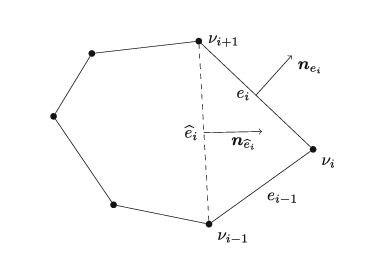
\includegraphics[width=0.5\textwidth]{figuras/Capítulo 4/4.6.png}
        \label{fig:4.6}

        {\small \textbf{Fonte:} \citet{virtualelementmethod50linesmatlab2017}}
    \end{figure}


    \indent Considerando uma forma bilinear $\mathcal{A}^{\Omega_v}(\cdot, \cdot)$ no elemento e uma função $v \in V$, o núcleo da forma bilinear é $\operatorname{ker}(\mathcal{A}^{\Omega_v}) = \{ v \in V : \mathcal{A}^{\Omega_v}(v, v) = 0 \}$. Para a base polinomial $\{\mathbf{p}_k\} \subset \mathbb{P}_k(\Omega_v)$, o núcleo é o espaço gerado pelos polinômios que anulam a forma bilinear: $\operatorname{ker}(\mathcal{A}^{\Omega_v}) = \operatorname{span}\{\mathbf{p}_1, \dots, \mathbf{p}_{n_{\operatorname{ker}}}\}$. \\
	\indent Como o projetor apresenta o mesmo operador diferencial que a forma bilinear, a condição de ortogonalidade define a projeção a menos de uma constante, condizente aos movimentos de corpo rígido. Portanto, as matrizes $\mathcal{G}^{(\nabla)}$ e $\mathcal{B}^{(\nabla)}$ possuem deficiência de posto (rank). \\
    \indent Contextualizando para o problema do projetor $\Pi_{k,*}^{(\nabla)}$, as linhas das matrizes $\mathcal{G}^{(\nabla)}$ e $\mathcal{B}^{(\nabla)}$ equivalem a um monômio. O operador gradiente anula os valores das linhas equivalentes aos monômios constantes e isso se agrava em relação à matriz $\mathcal{G}^{(\nabla)}$ porque esta se torna singular. Para eliminar a singularidade, introduz-se um operador de projeção adicional sobre as constantes, $P_0: V_k(\Omega_v) \rightarrow \mathbb{P}_0(E)$, que impõe a condição:
    
    \begin{equation}
        P_0(\Pi^\nabla v_h - v_h) = 0.
        \label{eq:4.31}
    \end{equation}

	\indent \citet{hitchhikersguidevirtualelementmethod2014a} apresenta algumas possibilidades para $P_0$, sendo elas:
    
    \begin{equation}
        P_0v_h := \begin{cases} \frac{1}{n_{\mathrm{nós}}} \sum_{i=1}^{n_{\mathrm{nós}}} v_h(V_i) \hspace{5mm} \text{para} \hspace{5mm} k = 1 \\ \frac{1}{|\Omega_v|} \int_{\Omega_v} v_h \hspace{5mm} \text{para} \hspace{5mm} k > 1 \end{cases}
        \label{eq:4.32}
    \end{equation}

    \fbox{\begin{minipage}{0.95\textwidth}
        \textbf{Exemplo 4.4.} Em um elemento triangular com dois graus de liberdade por nó está sendo calculado o projetor \(\Pi_2^{\nabla}\). Devido à deficiência de posto causada pela aplicação do gradiente, é necessário aplicar o operador \(P_0\). Determine os valores do projetor \(P_0\) para:

        \textbf{a)} \(p_5\) para a matriz \(\mathcal{G}^{(\nabla)}\).

        \textbf{b)} \(\varphi_4\) para a matriz \(\mathcal{B}^{(\nabla)}\).

        \textbf{c)} \(\varphi_{13}\) para a matriz \(\mathcal{B}^{(\nabla)}\).

        \hrulefill

        \textbf{Solução:}

        No elemento triangular de ordem \(k=2\) com \(n_{\rm dof\_nó}=2\), os graus de liberdade locais são ordenados da seguinte forma:

        - DOFs de contorno: índices 1 a 12;
        - DOFs internos (momentos constantes): índices 13 (direção \(x\)) e 14 (direção \(y\)).

        \textbf{a)} Para o monômio conjunto de monômios $$p_5 = xy$$ como \(k=2>1\), temos $$P_0(p_5) = \dfrac{1}{|\Omega_v|}\int_{\Omega_v} p_5 \,d\Omega = \dfrac{1}{|\Omega_v|}\int_{\Omega_v} xy \,d\Omega.$$ Esse valor, em geral, \textbf{não é nulo} e deve ser calculado explicitamente (via integração do monômio sobre o triângulo) e inserido na matriz \(\mathcal{G}^{(\nabla)}\).

        \textbf{b)} A função de base \(\varphi_4\) é um grau de liberdade de contorno. Para \(k>1\), desse modo, $P_0(\varphi_4) = 0.$


        \textbf{c)} A função de base \(\varphi_{13}\) corresponde ao momento interno constante na direção \(x\). Por construção dos graus de liberdade, $$P_0(\varphi_{13}) = \dfrac{1}{|\Omega_v|}\int_{\Omega_v} \varphi_{13} \,d\Omega.$$ Essa integral corresponde a um momento interno, então: $$\mathcal{B}_{1,13}^{(\nabla)} = 1 \quad \text{e} \quad \mathcal{B}_{2,13}^{(\nabla)} = 0 $$

    \end{minipage}}
    \vspace{5mm}

	\indent Com a inclusão da restrição de $P_0$, obtém-se a matriz de projeção elíptica na base polinomial: 
    
    \begin{equation}
        \{a\} = \Pi_{k,*}^\nabla = \left({\mathcal{G}^{(\nabla)}}\right)^{-1} \mathcal{B}^{(\nabla)}.
        \label{eq:4.33}
    \end{equation}

    \indent Um polinômio pode ser descrito tanto como uma expansão de bases polinomiais: $$p(x) = \sum_{i=1}^{2n_k} p_\alpha (x) a_\alpha.$$ Como também pode ser descrito através das bases nodais: $$p(x) = \sum_{i=1}^{2n_k} \varphi_i (x) d_i.$$ Para converter o projetor da base polinomial para a base canônica é realizado um mapa do espaço de solução sobre si: $$\Pi^{\nabla}: V_k(\Omega_v) \rightarrow V_k(\Omega_v).$$ A conversão da base polinomial para a base canônica é feita através da matriz $\mathcal{D}$.\\
    \indent A matriz $\mathcal{D}$ compreende dos valores que os polinômios utilizados na base assumem nos graus de liberdade do elemento. Para a conversão da base polinomial para a base nodal é realizada pela matriz $\mathcal{D}$ e o funcional dos graus de liberdade $\chi_i$ sobre os polinômios da base $p_\alpha$:
    
    \begin{equation}
        \mathcal{D}_{i\alpha} = \chi_i(p_\alpha) \hspace{5mm} \forall \hspace{5mm} i \in \{1, \ldots, n_{\mathrm{dof}} \}, \, \alpha \in \{ 1, \ldots, 2n_k \}.
        \label{eq:4.34}
    \end{equation}

    \vspace{5mm}
    \fbox{ \begin{minipage}{0.8\textwidth} 
        \textbf{Exemplo 4.5.} Em um polígono com 5 vértices e aproximação $k=1$, com as coordenadas $(5,0)$, o elemento possui diâmetro igual a 4 e a coordenada do centróide é (2,3). Determine o valor de $\mathcal{D}$ para o monômio $p_2 = \left(\frac{x - \bar{x}}{h_E}\right)$ no terceiro grau de liberdade. \\
        
        \hrulefill

        Solução: 

        Para $\mathcal{D}_{23}$:  $$\chi_3\left(p_2\right) = \left(\frac{x - \bar{x}}{h_E}\right) = \left(\frac{5 - 2}{4}\right) = \frac{3}{4}$$

    \end{minipage} }
    \vspace{5mm}

    \indent A relação entre os graus de liberdade $\vartheta_i$ e os coeficientes $a_\alpha$ é expressa por: 
    
    \begin{equation}
        \vartheta_i = \chi_i(p) = \chi_i \left( \sum_{\alpha=1}^{2n_k} p_\alpha (x) a_\alpha \right).
        \label{eq:4.35}
    \end{equation}

    \indent Através das propriedades de linearidade do funcional $\chi_i$:
    
    \begin{equation}
        \vartheta_i = \chi_i(p) = \sum_{\alpha=1}^{2n_k} a_\alpha \chi_i \left( p_\alpha (x) \right) \Leftrightarrow \vartheta_i = \sum_{\alpha=1}^{2n_k} a_\alpha \mathcal{D}_{i\alpha}.
        \label{eq:4.36}
    \end{equation}

    \indent Portanto, o operador de projeção mapeado para a base de graus de liberdade nodais fica definido por: 
    
    \begin{equation}
        \Pi_{k,0}^\nabla = \mathcal{D} \Pi_{k,*}^\nabla
        \label{eq:4.37}
    \end{equation}

    \indent Uma notável relação entre as matrizes $\mathcal{D}^{(\nabla)}$, $\mathcal{B}^{(\nabla)}$ e $\mathcal{G}^{(\nabla)}$ é:

    \begin{equation}
        \mathcal{G}_{\alpha,\beta}^{(\nabla)} = \left(\mathcal{B}^{(\nabla)}\mathcal{D}^{(\nabla)}\right)_{\alpha\beta}
        \label{eq:4.38}
    \end{equation}

    \vspace{5mm}
    \fbox{ \begin{minipage}{0.8\textwidth} 
        \textbf{Exemplo 4.5.} Demonstre a identidade $\mathcal{G}_{\alpha,\beta}^{(\nabla)} = \left(\mathcal{B}^{(\nabla)}\mathcal{D}^{(\nabla)}\right)_{\alpha\beta}$ 
        
        \hrulefill

        Solução: 

        Para $\alpha = 1:2$: $$\sum_{i=1}^{n_{dof}} \mathcal{B}^{(\nabla)}_{1:2,i} \mathcal{D}^{(\nabla)}_{i,\beta} = \sum_{i=1}^{n_{dof}} P_0\varphi_i \chi_i(p_\beta) = P_0\left( \sum_{i=1}^{n_{dof}}\varphi_i \chi_i(p_\beta) \right) = P_0(p_\beta) = \mathcal{G}_{1:2,\beta}^{(\nabla)}$$

        Para $\alpha > 2$: $$\begin{aligned}
            \sum_{i=1}^{n_{dof}} \mathcal{B}^{(\nabla)}_{\alpha,i} \mathcal{D}^{(\nabla)}_{i,\beta} = \sum_{i=1}^{n_{dof}} (\nabla p_\alpha, \nabla \varphi_i)_{\Omega_v} \chi_i(p_\beta) = \\ \left(\nabla p_\alpha, \nabla \left(\sum_{i=1}^{n_{dof}} \chi_i(p_\beta) \varphi_i \right)\right)_{\Omega_v} =  (\nabla p_\alpha, \nabla p_\beta)_{\Omega_v}= \mathcal{G}_{\alpha,\beta}^{(\nabla)}
        \end{aligned}$$

    \end{minipage} }
    \vspace{5mm}

    \indent A partir dessa relação entre as matrizes é possível obter $\mathcal{G}^{(\nabla)}$ sem a utilização das técnicas de integração comentadas anteriormente.


\subsection{Projetor \texorpdfstring{$\Pi_{k-1}^{0}$}{Pi k 0}}
\label{sec:projetor-L2}

    \indent O projetor $\Pi_{k}^0$, em contrapartida, à $\Pi_{k}^\nabla$ que projeta o gradiente de $u_h$, realiza a projeção do campo de deslocamentos. Essa característica o torna ideal para aproximação dos termos de massa e de forças de corpo (termo fonte). Diferente de $\Pi_{k}^\nabla$ que realiza uma ortogonalização do tipo $H^1$, o projetor $\Pi_{k}^0$ vai executar uma ortogonalização do tipo $L^2$:
    
    \begin{equation}
        \int_{\Omega_v} (v_h - \Pi^0 v_h) p_k d\Omega_v = 0 
        \label{eq:4.39}
    \end{equation}

    \indent Expandindo a Equação~\ref{eq:4.39}: 
    
    \begin{equation}
        \int_{\Omega_v} \Pi^0(v_h) \, p_k d\Omega_v = \int_{\Omega_v} v_h \,p_k d\Omega_v .
        \label{eq:4.40}
    \end{equation}

    \indent Substituindo o projetor em termos da base polinomial $H_k^P(\xi, \eta)$: 
    
    \begin{equation}
        \left( \int_{\Omega_v} [H_k^P]^T H_k^P \, d\Omega \right) \{a\} = \int_{\Omega_v} [H_k^P]^T v_h \, d\Omega \implies \mathcal{H} \{a\} = \mathcal{Q} 
        \label{eq:4.41}
    \end{equation}

    \indent O lado esquerdo possui apenas termos polinomiais e é computável utilizando as técnicas de integração numérica comentadas anteriormente. Neste trabalho, a integração da matriz $\mathcal{H}$ é efetuada com a técnica de integração de momentos sobre polígonos arbitrários descrita em \citet{calculationarbitrarymomentspolygonsa}.\\
    \indent Na matriz $\mathcal{Q}$ (lado direito da Eq.~\ref{eq:4.41}), o teorema da divergência não pode ser aplicado. Para resolver a integração das funções virtuais $v_h$, utiliza-se o espaço de solução aumentado definido na Eq.~\ref{eq:4.10}. Os momentos internos fornecem o valor de $(v_h, p_k)_{\Omega_v}$ para monômios de grau até $k-2$. Para os termos de grau $k-1$ e $k$, aplica-se a propriedade do espaço estendido da Eq.~\ref{eq:4.10}: 
    
    \begin{equation}
        (\varphi,p_k)_{\Omega_v} = (\Pi_k^\nabla \varphi,p_k)_{\Omega_v}.
        \label{eq:4.42}
    \end{equation}

    \indent Dessa forma, a matriz $\mathcal{Q}$ é montada em blocos: 
    
    \begin{equation}
        \mathcal{Q}_{\alpha i} = \begin{cases} \left(\varphi_i,p_\alpha\right)_{\Omega_v} & \text{se} \quad 1 \leq \alpha \leq 2n_{k-2} \\ \left(\Pi_k^\nabla \varphi_i, p_\alpha\right)_{\Omega_v} & \text{se} \quad 2n_{k-2} + 1 \leq \alpha \leq 2n_k \end{cases}
        \label{eq:4.43}
    \end{equation}

    \indent O projetor na base de monômios é dado por: 
    
    \begin{equation}
        \Pi_{k,*}^0 = \mathcal{H}^{-1} \mathcal{Q}
        \label{eq:4.44}
    \end{equation}

\subsection{Projetor \texorpdfstring{$\Pi_{k-1}^{\epsilon}$}{Pi k-1 epsilon}}
\label{sec:projetor-de-deformacoes}

    \indent O projetor $\Pi_{k-1}^\epsilon$ foi proposto por \citet{arbitraryorder2dvirtualelementspolygonalmeshespartelasticproblem2017a} para problemas de elasticidade. Embora o operador $\Pi_k^\nabla$ aproxime o gradiente, a presença de termos de ordem $k$ induz a representação de modos rígidos. Buscando filtrar os movimentos de corpo rígido, o projetor $\Pi_{k-1}^\epsilon$ projeta diretamente o tensor de deformações no espaço de polinômios de ordem $k-1$: 

    \begin{equation}
        \begin{aligned} 
            \Pi : V_{h,\Omega_v} \longrightarrow \left[ \mathbb{P}_{k-1}(\Omega_v) \right]^2 \\ 
                u_h (\mathbf{x}) \rightarrow \Pi u_h(\mathbf{x}) 
        \end{aligned}.
        \label{eq:4.45}
    \end{equation}

    \indent Para construção desse operador de projeção é utilizada uma relação de ortogonalidade do tipo $L^2$ para as deformações:
    
    \begin{equation}
        \int_{\Omega_v} \Pi_{k-1}^\epsilon(v_h)^T \, p_{k-1} d\Omega_v = \int_{\Omega_v} \epsilon{(v_h)} \,p_{k-1} d\Omega_v 
        \label{eq:4.46}
    \end{equation}

    \indent De maneira análoga à expansão dos deslocamentos dada por $H_k^P$ na Eq.~\ref{eq:4.22}, a aproximação do tensor de deformações em problemas bidimensionais (em notação de Voigt) é composta por três componentes independentes ($\epsilon_{xx}, \epsilon_{yy}, \gamma_{xy}$). Consequentemente, a representação polinomial das deformações associa cada função de base a esses três termos no campo cinemático. Expandindo a representação polinomial:  
    
    \begin{equation}
        \left( \int_{\Omega_v} [H_{k-1}^P]^T H_{k-1}^P \, d\Omega \right) \{a\} = \int_{\Omega_v} (\boldsymbol{\epsilon}(v_h))^T H_{k-1}^P \, d\Omega \implies \mathcal{G}^{(\epsilon)} \{a\} = \mathcal{B}^{(\epsilon)} 
        \label{eq:4.47}
    \end{equation}

    \indent Ao contrário de $\Pi_k^0$, o termo à direita possui o operador diferencial de deformação $\boldsymbol{\epsilon}(v_h)$, permitindo a aplicação direta do teorema da divergência sem necessidade do espaço de soluções aumentado: 
    
    \begin{equation}
        (\epsilon{(v_h)},H_{k-1}^P(\xi,\eta))_{\Omega_v} = \int_{\Gamma_e} \left(H_{k-1}^P(\xi_j,\eta_j) \cdot N^{(e)} \right) \varphi_{i\vert{}\Gamma_e} d\Gamma - \int_{\Omega_v} \nabla \cdot (H_{k-1}^P(\xi_j,\eta_j)) \varphi_i d\Omega 
        \label{eq:4.48}
    \end{equation}
	
    \indent Em uma abordagem similar ao que foi feito para o projetor gradiente, a parcela do contorno é obtida da quadratura de Gauss-Lobatto\footnote{A tabela com os pontos e pesos se encontra no anexo A}. A matrix $\mathcal{B}^{(\epsilon)}$ é calculada como:

    \begin{equation}
        \mathcal{B}^{(\epsilon)}_{\alpha i} = \sum_{e=1}^{n_e}\frac{l_e}{2}\sum_{q=1}^{k+1}w_q \bigl[H_k^P(\xi_q,\eta_q)\bigr]_{\alpha}\,N^{(e)}\, \delta_{\ell_e(i),\,q}\;-\; |\Omega_v|\sum_{\beta=1}^{n_{k-2}} \psi_{\alpha\beta}\, \delta_{m(i),\,\beta}.
        \label{eq:4.49}
    \end{equation}

    \noindent onde $$\bigl[\nabla\cdot H_k^P\bigr] = \sum_{\beta=1}^{n_k-2} d_{\alpha\beta}  \int_{\Omega_v} p_\beta \varphi_i d\Omega,$$ igual ao que foi feito na Equação~\ref{eq:4.26}, mas $\psi_{\alpha\beta}$ contém os coeficientes do divergente ao invés do laplaciano.\\
    \indent Considerando que $H_{k-1}^P \in \left[\mathbb{P}_{k-1}(\Omega) \right]^3$, a componente normal $N^{(e)}$ é modificada para:

    \begin{equation}
        N^{(e)} = \begin{bmatrix} N_{xe} & 0 & N_{ye} \\ 0 & N_{xe}  & N_{ye} \end{bmatrix} 
        \label{eq:4.50}
    \end{equation}  

    \indent Devido à natureza da relação de ortogonalização utilizada no projetor $\Pi_{k-1}^\epsilon$, a relação entre $\mathcal{G} = \mathcal{B}\mathcal{D}$ é inválida. A obtenção da matriz $\mathcal{G}^{\epsilon}$ deve ser feita do mesmo modo que a matriz $\mathcal{H}$.  A implementação para avaliação do projetor segue os mesmos passos de $\Pi_k^\nabla$, porém sem a necessidade do operador de projeção de constantes $P_0$, porque o operador de deformação já elimina naturalmente os movimentos de corpo rígido com uma aproximação de $k-1$. Dessa maneira:
    
    \begin{equation}
        \Pi_{k-1}^\epsilon = {\mathcal{G}^{(\epsilon)}}^{-1} \mathcal{B}^{(\epsilon)}
        \label{eq:4.51}
    \end{equation}

    \indent A matriz $\mathcal{D}^{\epsilon}$ ainda deve ser obtida para as operações envolvidas no termo de estabilidade. \citet{arbitraryorder2dvirtualelementspolygonalmeshespartelasticproblem2017a} afirma que o cálculo da matriz $\mathcal{D}^{\epsilon}$ é feito da mesma maneira que $\mathcal{D}^{\nabla}$, usando $k$ ao invés de $k-1$. 

\section{Matrizes de rigidez e massa}

    \indent Duas propriedades essenciais para garantir a existência, unicidade e estabilidade da solução no MEV são a consistência e a estabilidade.
    \begin{enumerate}
        \item Consistência: Garante que a solução discreta seja exata quando a solução analítica for um polinômio de grau menor ou igual a $k$: 
        \begin{equation}
            a^{\Omega_v}(v_h,p) = a_h^{\Omega_v}(v_h,p) \hspace{5mm}p \in \mathbb{P}_k({\Omega_v}).
            \label{eq:4.52}
        \end{equation}
        \item Estabilidade: Garante a positividade da forma bilinear discreta no espaço de elementos virtuais (\citet{arbitraryorder2dvirtualelementspolygonalmeshespartelasticproblem2017a}). Para estabilidade existem duas constantes ao qual não possuem limites superior ou inferior, apenas devem existir. Portanto, a forma bilinear deve escalonar como a forma contínua: 
        \begin{equation}
            \alpha_* a^{\Omega_v}\left( v_h , v_h \right) \leq a_h^{\Omega_v}\left( v_h , v_h \right) \leq \alpha^* a^{\Omega_v}\left( v_h , v_h \right).
            \label{eq:4.53}
        \end{equation}
    \end{enumerate}

    \indent Das formulações elastodinâmicas, Eq.~\ref{eq:3.57}, definem-se as matrizes da massa e rigidez: 

    \begin{equation}
        [M] = \int_{\Omega_v} \rho \varphi \varphi d\Omega_v,
        \label{eq:4.54}
    \end{equation}
    e 
	\begin{equation}
        [K] = \int_{\Omega_v} \epsilon(\varphi) \mathbb{C} \epsilon(\varphi) d\Omega_v.
        \label{eq:4.55}
    \end{equation}
\subsection{Matriz de massa}

    \indent Para a matriz de massa elementar com densidade $\rho$ constante, substitui-se o campo de funções de base $\varphi$ pela decomposição descrita na Eq.~\ref{eq:4.3}: $$[M] = \rho\int_{\Omega_v} (\Pi_k^0 \varphi + (I - \Pi_k^0) \varphi) (\Pi_k^0 \varphi + (I - \Pi_k^0) \varphi) d\Omega_v$$
    
    \begin{equation}
        \begin{aligned} 
            [M]  = \rho \int_{\Omega_v}\Pi_k^0 \varphi \Pi_k^0 \varphi d\Omega_v +  2\rho \int_{\Omega_v}\Pi_k^0 \varphi  (I - \Pi_k^0) \varphi d\Omega_v + \\  \rho\int_{\Omega_v} (I - \Pi_k^0) \varphi  (I - \Pi_k^0) \varphi d\Omega_v 
        \end{aligned}
        \label{eq:4.56}
    \end{equation}

    \indent Devido à propriedade de ortogonalidade em $L^2$ do projetor $\Pi_k^0$, o termo cruzado é nulo. A matriz de massa se divide em um termo de consistência $[M]^{\text{cons}}$ e um termo de estabilização $[M]^{\text{stab}}$: 
    
    \begin{equation}
        [M] = \rho\int_{\Omega_v}\Pi_k^0(\varphi) \Pi_k^0(\varphi) d\Omega_v + \rho\int_{\Omega} (I - \Pi_k^0) \varphi (I - \Pi_k^0) \varphi d\Omega_v
        \label{eq:4.57}
    \end{equation}

    \indent O termo de consistência é avaliado por: $$[M]^{\text{cons}}_{ij} = \rho \int_{\Omega_v} (\Pi_k^0 \varphi)^T (\Pi_k^0 \varphi) \, d\Omega = \rho \sum_{\alpha=1}^{n_k} \sum_{\beta=1}^{n_k} (\Pi_{k,*}^0)_{\alpha i}^T (\Pi_{k,*}^0)_{\beta j} \int_{\Omega_v} [H_k^P]_\alpha^T [H_k^P]_\beta \, d\Omega$$
    
    \begin{equation}
        [M]^{\text{cons}} = \rho (\Pi_{k,*}^0)^T \mathcal{H}^0 \Pi_{k,*}^0 
        \label{eq:4.58}
    \end{equation}

    $$\mathrm{t} \quad \mathcal{t} \quad \mathbb{t} \quad \mathit{t} \quad \mathfrak{t} \quad t$$

    \indent Nota-se que não foi necessário um procedimento de integração para a solução da matriz de massa. \citet{hitchhikersguidevirtualelementmethod2014a} afirma que o termo de consistência deve ser computado de maneira exata enquanto o termo de estabilidade pode ser aproximado. \\
    \indent O resíduo $(I - \Pi_k^0)q$ atua como um filtro para funções polinomiais: sempre que $q\in\mathbb{P}_k(\Omega_v)$, tem-se $(I - \Pi_k^0)q = 0$. Uma consequência imediata é que o resíduo também se anula no contorno do elemento quando a função é polinomial, garantindo que a estabilização não interfira no teste de consistência (patch test) do elemento.\\
    \indent O termo de estabilidade da matriz de massa é, em princípio, dado pelo produto interno $L^2$ das componentes residuais:
    \begin{equation}
        [M]^{\rm stab}_{ij} =\rho\int_{\Omega_v}(I - \Pi_k^0)\varphi_i\,(I - \Pi_k^0)\varphi_j\,d\Omega_v=\rho\bigl((I - \Pi_k^0)\varphi_i\,,(I - \Pi_k^0)\varphi_j\bigr)_{\Omega_v}.
        \label{eq:4.59}
    \end{equation}
    \indent Como as funções virtuais não são conhecidas explicitamente no interior do elemento, esse produto interno não pode ser avaliado de forma exata. Substitui-se, então, a norma $L^2$ residual pela norma euclidiana dos graus de liberdade residuais. Essa substituição é justificada pela \emph{equivalência de normas} em espaços de dimensão finita: no núcleo do projetor $\ker(\Pi_k^0)$ existe uma constante $\alpha$ independente do tamanho do elemento tal que
    \begin{equation}
        \alpha_*\,\|v\|_{L^2(\Omega_v)}^2 \;\le\; \sum_{r=1}^{n_{\mathrm{dof}}}\bigl(\chi_r(v)\bigr)^2 \;\le\; \alpha^*\,\|v\|_{L^2(\Omega_v)}^2 \qquad \forall v\in\ker(\Pi_k^0).
        \label{eq:4.60}
    \end{equation}
    \indent A desigualdade~\eqref{eq:4.53} (propriedade de estabilização) garante que a forma bilinear 
    \begin{equation*}
        S(v,w)=\sum_{r=1}^{n_{\mathrm{dof}}}\chi_r(v)\,\chi_r(w)
    \end{equation*} 
    é equivalente ao produto interno $L^2$ no espaço residual. Além disso, as constantes de equivalência na desigualdade~\eqref{eq:4.60} dependem da medida do elemento (espaço de dimensão finita). Agrupando a densidade $\rho$, as constantes de escala do espaço e a medida do elemento (como a área $|\Omega_v|$ ou $h_e^2$) no coeficiente de escalonamento $\tau_m$ da formulação, o produto interno residual é aproximado por:
    \begin{align*}
        [M]^{\rm stab}_{ij}&=\rho\bigl((I - \Pi_k^0)\varphi_i\,,(I - \Pi_k^0)\varphi_j\bigr)_{\Omega_v}\\ \approx\tau_m\sum_{r=1}^{n_{\mathrm{dof}}}\chi_r\bigl((I - \Pi_k^0)\varphi_i\bigr)\,\chi_r\bigl((I - \Pi_k^0)\varphi_j\bigr).
    \end{align*}
    \indent Em forma matricial, essa expressão torna-se
    \begin{equation}
        [M]^{\rm stab}=\tau_m\bigl[(I - \mathcal{D}\Pi^0)^T(I - \mathcal{D}\Pi^0)\bigr].
        \label{eq:4.61}
    \end{equation}

    \indent Reunindo as parcelas, a matriz de massa elementar toma a forma:

    \begin{equation}
        [M] = d \left( \left(\Pi^0{k,*}\right)^T\mathcal{H}^0\Pi^0{k,*} + \tau_m\bigl[(I - \mathcal{D}\Pi^0)^T(I - \mathcal{D}\Pi^0)\bigr] \right),
        \label{eq:4.62}
    \end{equation}  

\subsection{Matriz de rigidez}	

    \indent O procedimento para a matriz de rigidez é semelhante ao que foi feito para a matriz de massa, substituindo a deformação ${\epsilon}(\varphi)$ por meio do projetor $\Pi_{k-1}^\epsilon$: 

    \begin{equation}
        [K]_{ij} = \int_{\Omega_v} (\boldsymbol{\epsilon}(\Pi_{k-1}^\epsilon \varphi_i))^T \mathbb{C} \boldsymbol{\epsilon}(\Pi_{k-1}^\epsilon \varphi_j) \, d\Omega + \int_{\Omega_v} \epsilon\left( (I - \mathcal{D}\Pi_{k-1}^\epsilon) \varphi_i \right)^T \mathbb{C} \epsilon\left( (I - \mathcal{D}\Pi_{k-1}^\epsilon) \varphi_j \right) d\Omega.
        \label{eq:4.64}
    \end{equation}

    \noindent Na Equação~\ref{eq:4.64} os termos cruzados já foram eliminados.\\
    \indent O termo de consistência é dado por:
    
    \begin{equation}
        [K]^{\text{cons}} = (\Pi_{k-1}^{\epsilon})^T \mathcal{G}^{(\epsilon)} \mathbb{C} \, \Pi_{k-1}^{\epsilon}
        \label{eq:4.65}
    \end{equation}

    \indent O termo de estabilidade é:  $$[K]_{ij}^{Stab} = \int_{\Omega_v} (I - \mathcal{D}\Pi_{k-1}^{\epsilon})\epsilon\left(\varphi_i \right)^T \mathbb{C} (I - \mathcal{D}\Pi_{k-1}^{\epsilon})\epsilon\left(\varphi_j \right)^T  d\Omega.$$
    \indent Como visto na equação Eq.~\ref{eq:4.59}, o termo $(I - \mathcal{D}\Pi_{k-1}^{\epsilon})$ não é computável pelas dimensões de $\mathcal{D}$ e $\Pi^{\epsilon}$ não serem compatíveis. O termo de consistência e o termo de estabilidade são desacoplados entre si, desse modo o termo de estabilidade pode ser aproximado por\footnote{No exemplo 4.7 será realizada a demonstração dessa propriedade. A demonstração é baseada nas provas encontradas no trabalho de \citet{basicprinciplesvirtualelementmethods2013a}.}: 

    \begin{equation}
        [K]^{\text{Stab}} = \tau_k (I - \mathcal{D}\Pi_{k}^\nabla)^T (I - \mathcal{D}\Pi_{k}^\nabla),
        \label{eq:4.66}
    \end{equation}

    \noindent onde $\tau_k$ é coeficiente de escalonamento da parcela elástica da equação diferencial.\\ 
    \indent Uma forma alternativa para o termo de estabilização é sugerida por \citet{arbitraryorder2dvirtualelementspolygonalmeshespartelasticproblem2017a}. Essa estabilização se baseia em um projetor complementar construído unicamente com a matriz $D$:

    \begin{equation}
        [K]^{\text{Stab}} = \tau_k \left[ I - D (D^T D)^{-1} D^T \right].
        \label{eq:4.67}
    \end{equation}

    \indent A matriz de rigidez elementar completa é expressa por: 
    
    \begin{equation}
        [K] = (\Pi_{k-1}^\epsilon)^T \mathcal{G}^{(\epsilon)} \Pi_{k-1}^\epsilon + (I - \mathcal{D}\Pi_{k-1}^\epsilon)^T \tau_k (I - \mathcal{D}\Pi_{k-1}^\epsilon) 
        \label{eq:4.68}
    \end{equation}

    \fbox{ \centering\begin{minipage}{.9\textwidth} 
        \textbf{Exemplo 4.6.} Prove que os termos de consistência e de estabilidade são desacoplados.
        
        \hrulefill

        \indent A forma bilinear discreta em um domínio $K$ é: $$a_h^{\Omega_v}(v_h,q) = \int_K \mathbb{C}\Pi_{k-1}^0(\epsilon(v_h)) : \Pi_{k-1}^0(\epsilon(q))  dK + S_a^{\Omega_v}(v_h,q).$$ $S_a^{\Omega_v}(v_h,q)$ é uma notação simplificada para o termo de estabilidade.\\
        \indent Da propriedade de consistência, a forma bilinear discreta deve ser rigorosamente igual à forma bilinear contínua.\\
        \indent Para uma função $q \in \left[\mathbb{P}_k(K)\right]^2$, para um projetor $\Pi^0_{k-1}$ a identidade é válida: $$\Pi^0_{k-1}(\epsilon(q))=\epsilon(q).$$ Utilizando a propriedade de ortogonalidade  do projetor $L^2$: $$\int_K \mathbb{C}\Pi_{k-1}^0(\epsilon(v_h)) : \Pi_{k-1}^0(\epsilon(q) dK = \int_K \mathbb{C}\epsilon(v_h) : \epsilon(q) dK = a^{\Omega_v}(v_h,q).$$
        \indent Para que a consistência existe, a parcela de estabilidade deve se anular. Considerando que o termo não polinomial é nulo quando a ele é aplicada uma função polinomial, é possível concluir que: $$(I - \Pi_{k-1}^0)\epsilon(q) = 0 \therefore S_a^{\Omega_v}(v_h,q) = 0 \hspace{3mm} \forall q \in \left[\mathbb{P}_k(K)\right]^2.$$
        \indent Assim como $\Pi^0_{k-1}$, o operador $\Pi^\nabla_k$ por definição é um operador sobre $\left[\mathbb{P}_k(K)\right]^2$ agindo como identidade de $q$ nesse espaço: $$\Pi^\nabla_k q = q \hspace{3mm} \forall q \in \left[\mathbb{P}_k(K)\right]^2.$$ Assim, a relação: $$(I - \Pi^\nabla_k)q = 0$$ é verdadeira. Intuindo isso, chega-se a conclusão de que: $$\int_K \mathbb{C}(I-\Pi_{k-1}^0)\epsilon(v_h) : (I-\Pi_{k-1}^0)\epsilon(q) dK = \int_K \mathbb{C}(I-\Pi_{k}^\nabla)v_h : (I-\Pi_{k}^\nabla)q dK = 0.$$ Destarte provando o desacoplamento dos termos de consistência e estabilidade.
    \end{minipage} }
    \vspace{5mm}

    \subsection{Os parâmetros de estabilização}

    \indent Os coeficientes de escalonamento são amplamente debatidos na literatura porque são altamente dependentes do problema, o que motivou o desenvolvimento de formulações de elementos virtuais livres de estabilização. Para problemas de elasticidade, algumas formas encontradas na literatura de se obter o coeficiente $\tau_k$ são apresentadas a seguir.

    \paragraph{Fator de escala original ou uniforme ($\max_i (K_{C_{i,i}})$)} Criado por \citet{basicprinciplesvirtualelementmethods2013a}, busca impedir que o elemento se deforme livremente sem gerar esforço interno (modos de energia nula). Para isso, penaliza essas deformações irreais aplicando um mesmo coeficiente a todos os graus de liberdade. Este método não está atrelado a um problema específico e garante que a matriz de estabilização possua as mesmas proporções da matriz de consistência. No entanto, em polígonos irregulares, aplicar o maior escalar penaliza uniformemente todas as direções de forma severa.

    \paragraph{Fator de escala físico ($\max(2\mu, \lambda)$)} Foi desenvolvido por \citet{virtualelementslinearelasticityproblems2013} para evitar o problema de travamento volumétrico numérico em materiais quase incompressíveis, frequentemente causado pelo escalonamento uniforme. Sua formulação depende unicamente das características elásticas do material (com $\mu$ e $\lambda$ sendo os parâmetros de Lamé), o que mantém as unidades físicas consistentes e possui interpretação direta. É comumente utilizado na solução de problemas elastodinâmicos, como visto em \citet{antonietti2020virtual}.

    \paragraph{Fator de escala pelo traço ($\alpha_0 \text{tr}(K_C)$)} Usa o traço da parcela consistente da matriz de rigidez calibrado por um coeficiente $\alpha_0$ definido pelo usuário. \citet{arbitraryorder2dvirtualelementspolygonalmeshespartelasticproblem2017a} recomendam a utilização de $\alpha_0 = 0,5$ em problemas de elasticidade linear bidimensionais. Embora apresente os mesmos problemas de travamento numérico que o escalonamento uniforme, é frequentemente utilizado junto à estabilização de energia (Eq.~\ref{eq:4.67}).

    \paragraph{Fator de escala D-Recipe ($\text{diag}(\vert{}K_{C_{i,i}}\vert{})$)} Proposta por \citet{beiraodaveiga2017high} (referida como ``diagonal recipe''), esta abordagem substitui o uso de um parâmetro escalar uniforme que pode ser inadequado para aproximações de grau elevado (alto $k$), especialmente em três dimensões, onde diferentes funções de base podem carregar níveis de energia muito distintos. A D-Recipe utiliza uma matriz diagonal cujos termos são calculados com base nos valores da diagonal da matriz de consistência. Dessa forma, em vez de penalizar o elemento com um escalar uniforme que pode gerar super-rigidez, a formulação cria uma estabilização que acompanha a rigidez e a energia de cada função de base direcionalmente.

    \paragraph{Fator de escala D-Recipe híbrido ($\max\left([K_{E,c}]_{ii}, \alpha_0 \frac{\text{tr}(\mathbb{C})}{n_C}\right)$)} Esta formulação aplica prioritariamente o valor da diagonal da matriz de consistência, mas impõe um limite inferior para esses termos baseado no traço da matriz de elasticidade (ou matriz constitutiva) $\mathbb{C}$. Esse limite inferior é adotado porque a rigidez obtida apenas pelo termo de consistência ($[K_{E,c}]_{ii}$) pode se tornar excessivamente pequena em elementos altamente não convexos que possuem muitos nós. Na equação, o termo é calibrado por um parâmetro adimensional $\alpha_0$ definido pelo usuário, e $n_C$ representa a dimensão (tamanho) da matriz de elasticidade $\mathbb{C}$ (\citet{nonconvexmesheselastodynamicsusingvirtualelementmethodsexplicittimeintegration2019a}). Para problemas de elastodinâmica com integração temporal explícita, os valores recomendados para o parâmetro $\alpha_0$ são $1/3$ em problemas bidimensionais e $1/9$ em problemas tridimensionais(\citet{numericalrecipeselastodynamicvirtualelementmethodsexplicittimeintegration2020}).

    \vspace{1em}
    \indent Para o coeficiente $\tau_m$ utilizado na estabilização da matriz de massa, existe pouca documentação sobre diferentes maneiras de se calcular o parâmetro. Na literatura, o termo corresponde à massa do elemento, sendo frequentemente calculado como o produto da massa específica $\rho$ pela área do elemento (\citet{numericalrecipeselastodynamicvirtualelementmethodsexplicittimeintegration2020}) ou pelo quadrado do diâmetro do elemento (\citet{antonietti2020virtual}).  

\section{Considerações finais}

    \indent O algoritmo~\ref{alg:typical_vem} apresenta-se a estrutura para o cálculo dos projetores e montagem das matrizes de rigidez e massa em uma formulação do MEV: 

        \begin{algorithm}[htpb!]
        \caption{Implementação do método dos elementos virtuais}
        \label{alg:typical_vem}
        \begin{algorithmic}[1]
    
        \Require malha, condições de contorno, $[\mathbb{C}]$, $\rho$, $k$, $d$, $\tau_k$ e $\tau_m$
        \State inicializar a matriz de rigidez e matriz de massa global.
        \While{cada elemento $\Omega_v$ na malha}
            \State Determine $|\Omega_v|$, $n_v$, $h$, $(\bar{x},\bar{y})$, $le$, $\{\mathbf{n}_{e}\}$
            \State $(\xi, \eta) \leftarrow \left(\frac{x-\bar{x}}{h}, \frac{y-\bar{y}}{h}\right)$
    
            \Comment{Operadores do projetor $\nabla$ e $\epsilon$}

            \State $[\mathcal{B}^{\nabla}] \leftarrow a_{\Omega_v}^{\nabla}(\varphi, H_k^P)$ \hfill Eq.~\ref{eq:4.32}
            \State $[\mathcal{B}^{\epsilon}] \leftarrow a_{\Omega_v}^{\epsilon}(\varphi, H_{k-1}^P)$ \hfill Eq.~\ref{eq:4.48}
            \State $[\mathcal{D}^{\nabla}] \leftarrow \chi(H_k^P)$ \hfill Eq.~\ref{eq:4.34}
            \State $[\mathcal{G}^{\nabla}] \leftarrow [\mathcal{B}^{\nabla}][\mathcal{D}^{\nabla}]$ \hfill Eq.~\ref{eq:4.38}
            \State $[\mathcal{G}^{\epsilon}]  \leftarrow \mathbf{\int_{\Omega_v} \,H_{k-1}^P \, H_{k-1}^P \, d{\Omega_v}}$ \hfill Eq.~\ref{eq:4.48}
            \State $[\mathbf{\Pi}^{\nabla}] \leftarrow [\mathcal{G}^{\nabla}]^{-1}[\mathcal{B}^{\nabla}]$ \hfill Eq.~\ref{eq:4.24}
            \State $[\mathbf{\Pi}^{\epsilon}] \leftarrow [\mathcal{G}^{\epsilon}]^{-1}[\mathcal{B}^{\epsilon}]$ \hfill Eq.~\ref{eq:4.49}

            \Comment{Cálculo da Matriz de Rigidez}

            \State $[\mathbf{k}_{\Omega_v}^C] \leftarrow [\mathbf{\Pi}^{\epsilon}]^T [\mathcal{G}^{\epsilon}] [\mathbf{\mathbb{C}}] [\mathbf{\Pi}^{\epsilon}]$ \hfill Eq.~\ref{eq:4.65}
            \State $[\mathbf{k}_{\Omega_v}^S] \leftarrow \tau_k ([\mathbf{I}] - [\mathcal{D}^{\nabla}][\mathbf{\Pi}^{\nabla}])^T ([\mathbf{I}] - [\mathcal{D}^{\nabla}][\mathbf{\Pi}^{\nabla}])$ \hfill Eq.~\ref{eq:4.66}
            \State $[\mathbf{k}_{\Omega_v}] \leftarrow d \left( [\mathbf{k}_{\Omega_v}^C] + [\mathbf{k}_{\Omega_v}^S] \right)$ \hfill Eq.~\ref{eq:4.68}
    
            \Comment{Operadores do projetor $L^2$ e Cálculo da Matriz de Massa}

            \State $[\mathcal{H}^0] \leftarrow \mathbf{\int_{\Omega_v} H_k^P \, H_k^P \, d{\Omega_v}}$ 
            \State Montar blocos de $[\mathbf{Q}]$ \hfill Eq.~\ref{eq:4.43}
            \State $[\mathbf{\Pi}^0] \leftarrow [\mathbf{H}^0]^{-1}[\mathcal{Q}]$ \hfill Eq.~\ref{eq:4.44}
    
            \State $[\mathbf{M}_{\Omega_v}^C] \leftarrow \rho [\mathbf{\Pi}^{0}]^T [\mathbf{H}^{0}] [\mathbf{\Pi}^{0}]$ \hfill Eq.~\ref{eq:4.61}
            \State $[\mathbf{M}_{\Omega_v}^S] \leftarrow \tau_m ([\mathbf{I}] - [\mathcal{D}^{\nabla}][\mathbf{\Pi}^{0}])^T ([\mathbf{I}] - [\mathcal{D}^{\nabla}][\mathbf{\Pi}^{0}])$ \hfill Eq.~\ref{eq:4.61}
            \State $[\mathbf{M}_E] \leftarrow d \left( [\mathbf{M}_{\Omega_v}^C] + [\mathbf{M}_{\Omega_v}^S] \right)$ \hfill Eq.~\ref{eq:4.62}
    
            \State Juntar $[\mathbf{k}_{\Omega_v}]$ e $[\mathbf{M}_{\Omega_v}]$ em suas corretas posições nas matrizes globais 
        \EndWhile
        \end{algorithmic}
    \end{algorithm}

    \indent O valor de $u_h$ não é plenamente obtido ao final do processo por conter uma parcela virtual, contudo ele pode ser aproximado de modo aceitável apenas pela parcela polinomial: 

    \begin{equation}
        u_h = H_k^P (\xi,\eta) \Pi_{k,*}^0 \{u_e\} 
        \label{eq:4.69}
    \end{equation}

    \indent Para o gradiente de deslocamentos, tem-se: 

    \begin{equation}
        \nabla u_h = \nabla H_k^P (\xi,\eta) \Pi_{k,*}^{\nabla} \{u_e\} 
        \label{eq:4.70}
    \end{equation}

    \indent As deformações podem ser aproximadas diretamente pelo operador $\Pi_{k-1}^{\epsilon}$ da mesma maneira feita para $u_h$. O vetor de deformações é dado por: 
    
    \begin{equation}
        \epsilon(u_h) = H_{k-1}^P (\xi,\eta) \Pi_{k-1,*}^{\epsilon} \{u_e\}
        \label{eq:4.71}
    \end{equation}

    \indent Recordando alguns conceitos vistos no Capítulo~\ref{cap:2}: tal qual o MEF em sua formulação clássica, também é necessária a utilização dos procedimentos de recuperação de tensões para o MEV. Para se ter uma aproximação de $u_h$ e $\epsilon(u_h)$ considerando a utilização do termo não polinomial, é necessário a aplicação de técnicas de recuperação de funções na etapa de pós-processamento.

    